\documentclass{article}

\usepackage[utf8]{inputenc}

% Packages
\usepackage{amsmath,amssymb}
\usepackage{bm}% boldmath
\usepackage{listings} % Code block (source code) \begin{lstlisting} 
\usepackage{natbib}
\usepackage{graphicx}
\usepackage{lmodern}
\usepackage[usenames,dvipsnames,svgnames,table]{xcolor}
\usepackage[textwidth=16cm,textheight=23cm]{geometry}

%\usepackage{inconsolata} % New monospace font

% URL
\usepackage{url}
\usepackage[colorlinks=true, a4paper=true, pdfstartview=FitV, linkcolor=blue, citecolor=blue, urlcolor=blue]{hyperref}

% Figures
\usepackage[font=small, labelfont=bf]{caption}
\usepackage{subfig} % Subfigures. Uses \subfloat[captions text]{figure}

% Tables
\usepackage{booktabs}   % Allows the use of \toprule, \midrule and \bottomrule in tables for horizontal lines
\newcommand{\ra}[1]{\renewcommand{\arraystretch}{#1}} % spaces in tables

% Itemize
\usepackage{enumitem}

% Commands
%\newcommand{\code}[1]{\texttt{#1}} % \code{inline code}
\newcommand{\code}[1]{{\small\ttfamily #1}} % \code{inline code}
\newcommand{\expval}[1]{\langle #1 \rangle} %
\renewcommand{\theequation}{\arabic{section}.\arabic{equation}} % Book format equation
\renewcommand{\thefigure}{\arabic{section}.\arabic{figure}} % Book format figure
\renewcommand{\vec}[1]{{\bf #1}} % Lars likes this better than arrow

% Set page attribution
\setlength{\parindent}{0pt}


% PSTRICKS
\usepackage{pstricks,pst-node,pst-tree} % includes graph additions
\usepackage{pst-pdf} % Compiles the pictures
\usepackage{pst-node}
\usepackage{pst-plot}
\usepackage{pst-3dplot}
%\usepackage{pstricks-add,babel}




\lstset{
language=Python,                        % Code langugage
commentstyle=\color{gray},              % Comments font
basicstyle=\small\ttfamily,             % Code font, Examples: \footnotesize, \ttfamily
keywordstyle=\bfseries\color{blue},
stringstyle=\color{orange},
numbers=left,                           % Line nums position
numberstyle=\tiny,                      % Line-numbers fonts
stepnumber=1,                           % Step between two line-numbers
numbersep=5pt,                          % How far are line-numbers from code
frame=none,                             % A frame around the code
tabsize=4,                              % Default tab size
captionpos=b,                           % Caption-position = bottom
breaklines=true,                        % Automatic line breaking?
breakatwhitespace=false,                % Automatic breaks only at whitespace?
showspaces=false,                       % Dont make spaces visible
showstringspaces=false,                 % Dont make spaces visible in strings
showtabs=false,                         % Dont make tabls visible
belowskip=8pt,
morekeywords={range, xrange},
% backgroundcolor=\color{yellow}
% emph={[2]root,base}
% morekeywords={one,two,three,four,five,six,seven,eight,
}


%commentstyle=\color{gray},              % Comments font
%basicstyle=\small,                      % Code font, Examples: \footnotesize, \ttfamily



%basicstyle=\footnotesize\ttfamily,
%keywordstyle=\bfseries\color{green!40!black},
%commentstyle=\itshape\color{purple!40!black},
%identifierstyle=\color{blue},
%stringstyle=\color{orange},







% ***************************************************
% HEADER INFORMATION

\title{Exercise 3}
\author{Molecular Statistics, Week 3}
\date{2014}

% ***************************************************

\begin{document}


% ***************************************************
% BEGIN DOCUMENT
% ***************************************************

\maketitle


\section{Introduction and Theory}

In this exercise you are going to implement a simulation of a 2D Lennard-Jones potential.
Figure \ref{fig:potentials} shows the three different potentials we've encountered so far.

\begin{figure}[h!]
\begin{center}
    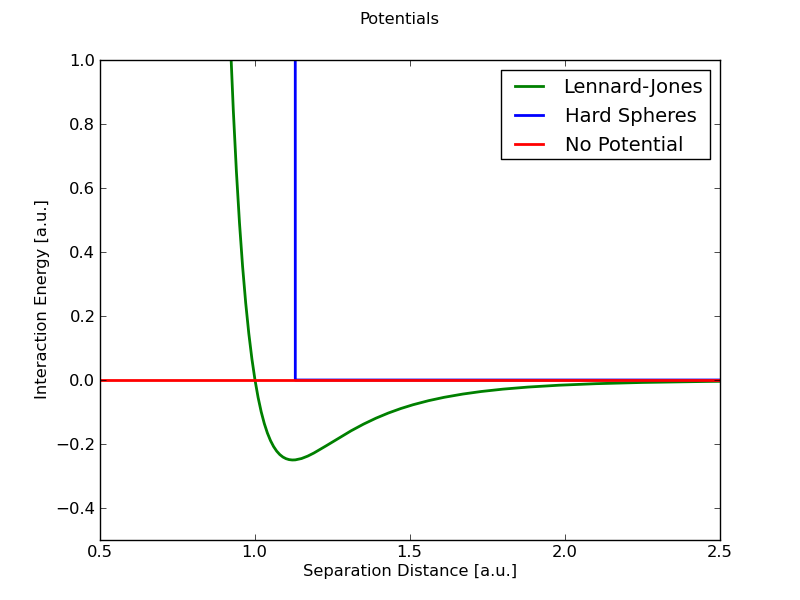
\includegraphics[width=0.75\textwidth]{potentials.png}
    \caption{The three different potentials we've encountered so far.}
    \label{fig:potentials}
\end{center}
\end{figure}


\subsection{The Lennard-Jones potential energy}

The Lennard-Jones potential energy between two interacting particles $i$ and $j$ is given by:

\begin{equation}
    U_{ij} = 4 \epsilon \left[ \left(\frac{\sigma}{r_{ij}} \right)^{12} - \left(\frac{\sigma}{r_{ij}} \right)^6 \right]
\end{equation}

Here $r_{ij}$ is the distance between the two particles. For simplicity, we
set $\epsilon = 1$ and $\sigma = 1$, in which case the energy is reduced
to:

\begin{equation}
    U_{ij} = 4 \left[ \left(\frac{1}{r_{ij}} \right)^{12} - \left(\frac{1}{r_{ij}} \right)^6 \right]
\end{equation}

The total potential energy of the system is then:

\begin{equation}
    U_{\mathrm{Total}} = 4 \sum_{i>j} \left[ \left(\frac{1}{r_{ij}} \right)^{12} - \left(\frac{1}{r_{ij}} \right)^6 \right]
\end{equation}

You should now be able to see how the summation $\sum_{i>j}$ requires a double
loop over all particles in your code. These usually look
something like:

\begin{lstlisting}[language=python]
energy = 0.0
for i in range(n_particles):
    for j in range(n_particles):
        if i > j:
            energy = energy + ...
\end{lstlisting}

\subsection{Inter-particle forces in the Lennard-Jones potential}

In the past two exercises, the total momentum of the particles was conserved.
In the Lennard-Jones potential, however, we must calculate the force exerted by
the particles upon each other, and use the forces to update the positions and
velocities of the particles.
First, recall how we are able to calculate the force \textbf{F} using the
energy gradient:

\begin{equation}
    \mathbf{F} = -\nabla U = -\left( \frac{\partial U}{\partial x_1},\ \frac{\partial U}{\partial y_1},\  \frac{\partial U}{\partial x_2},\ \frac{\partial U}{\partial y_2},\ \ldots\ ,\frac{\partial U}{\partial x_n},\ \frac{\partial U}{\partial y_n}\right)
    \label{eq:force}
\end{equation}

The $x$-components of the force between two interacting particles $i$ and $j$
are:

\begin{align}
-\frac{\partial}{\partial x_i} U_{ij} &= -48\ \frac{x_j - x_i}{r^2_{ij}}\left[ \left(\frac{1}{r_{ij}} \right)^{12} - 0.5 \left(\frac{1}{r_{ij}} \right)^6 \right] \\
-\frac{\partial}{\partial x_j} U_{ij} &=  48\ \frac{x_j - x_i}{r^2_{ij}}\left[ \left(\frac{1}{r_{ij}} \right)^{12} - 0.5 \left(\frac{1}{r_{ij}} \right)^6 \right]
\end{align}

The $y$-components are, of course, similar.

\subsection{The Velo-Verlet solver}

%TODO Reference to Jan's slides

The Velocity Verlet (Velo-Verlet) solver is one of many ways to go about
integrating the motion of particles. The Velo-Verlet algorithm
updates the forces, velocities and positions at the same time step. The
Velo-Verlet equations for integrating the positions and velocities are (in the
$x$-direction for one particle):

\begin{eqnarray}
x(t + dt) &=& x(t) + dt\ v_x(t) + 0.5\ dt^2\ a_x(t) \label{eq:velo_pos} \\\
v_x(t + dt) &=& v_x(t) + 0.5\ dt \left[a_x(t) + a_x(t+dt)\right] \label{eq:velo_vel}
\end{eqnarray}

In the program you will be implementing today, we will set the mass of the particles
to 1, so the value of the acceleration is equal to the value of the
force.

Let's recap: The Velo-Verlet algorithm uses the forces,
velocities and positions from the current position to calculate the forces,
velocities and positions after the next time-step. In short it is a three-step
procedure:

\begin{enumerate}
    \item Calculate new positions using Eq. \ref{eq:velo_pos}
    \item Calculate new forces using Eq. \ref{eq:force}
    \item Calculate new velocities using Eq. \ref{eq:velo_vel}
\end{enumerate}

The resulting forces, velocities and particle positions are then saved as input
for the next Velo-Verlet integration step.


\newpage
\clearpage
\section{Exercises}

Before you begin, inspect your code from last week. It should more or less
contain the following functionality:

% TODO ADD FROM SOLUTION WEEK 2!

\begin{lstlisting}[language=python]
import random
import matplotlib.pyplot as plt
import numpy as np
import video # 2D video creator

def distance(xi,yi,xj,yj):
    """ Calculate the distance between particle i and particle j """
    dx = xj-xi
    dy = yj-yi
    return np.sqrt(dx**2 + dy**2)


def initialize_particles(n_particles, box_width):
    """ initialize particles, positions and velocities for n_particles """
    return x_positions, y_positions, x_velocities, y_velocities


def take_step(x_positions, y_positions, x_velocities, y_velocities, dt):
    """ Simulate particle movement from their positions and velocities in a
    single time-step dt """
    return x_positions, y_positions, x_velocities, y_velocities


# Define simulation
box_with    = 10
n_particles = 20
n_steps     = 1000
dt          = 0.001

# Initialize particles
X, Y, Vx, Vy = initialize_particles(n_particles)

# Take steps
for n in range(n_steps):
    X, Y, Vx, Vy = take_step(X, Y, Vx, Vy, dt)

    if n % 10 == 0:
        video.add_frame(X, Y)

video.save('week3')

\end{lstlisting}

\newpage
\clearpage


Firstly, you will need to write the relevant code/functions to calculate the
Lennard-Jones potential energy for a given system.

\begin{enumerate}
    % Make them use solution, or try to continue from their own code?
    \item Save the solution from last week in a new file which you will be using today.
        {\em Note:} Remember to call it something new, e.g. \code{exercise\_3.py}.


    \item Write a function called \code{lennard\_jones} that takes the lists of $x$- and $y$-coordinates as arguments and returns the Lennard-Jones energy. Use the code below as inspiration.
\begin{lstlisting}[language=python]
def lennard_jones(x_positions, y_positions, n_particles):
    """ Calculates the energy of the LJ potential """
    energy = 0.0
    for i in range(n_particles):
        for j in range(n_particles):
            if (i > j):
                energy = energy + ...

    return energy
\end{lstlisting}

\end{enumerate}

When you think you have written the Lennard-Jones energy function properly,
it's time to test whether your function works correctly or not.
Define two lists:

\begin{lstlisting}[language=python]
n_particles = 2
X_test = [0.0, 0.0]
Y_test = [0.0, 1.4]
\end{lstlisting}


\begin{enumerate}
    \setcounter{enumi}{2}

    \item Now call the Lennard-Jones energy function with the two lists as
        arguments and print the result. If your energy function works, the
        resulting energy should be -0.4607.

\end{enumerate}

Next, you will extend the Lennard-Jones function to also calculate
the forces. In our 2D system the force has $x$- and $y$-components for each
particle.
So for this it would be natural to extend your code to store the $x$- and
$y$-components in two lists called \code{x\_force} and \code{y\_force}, just
like the velocities.

\begin{enumerate}
    \setcounter{enumi}{3}

    \item Extend your Lennard-Jones function to \textit{also} return the forces.
        Use the code below for inspiration.

\begin{lstlisting}[language=python]
def lennard_jones(x_positions, y_positions, n_particles):
    energy = 0.0

    x_force = [0.0 for i in range(n_particles)]
    y_force = [0.0 for i in range(n_particles)]

    for i in range(n_particles):
        for j in range(n_particles):
            if (i > j):
                energy = energy + ...

                x_force[i] = x_force[i] + ...
                y_force[i] = y_force[i] + ...

                x_force[j] = x_force[j] + ...
                y_force[j] = y_force[j] + ...

    return x_force, y_force, energy

\end{lstlisting}

    \item Use the \code{X\_test} and \code{Y\_test} lists from the previous question and
        calculate the forces and energies.
        If your code returns \code{x\_force[0]} = 0.0 and \code{y\_force[0]} = 1.6720, your
        code might be working as it should.

\end{enumerate}

\newpage

Next is to implement the Velo-Verlet solver.
The Velo-Verlet solver needs the current forces, velocities and
particle positions as input. Your code already initializes the
velocities and positions, but doesn't calculate the initial forces. \\

Last week we used random $x$- and $y$-coordinates.
It's not a good idea, however, to use random X-coordinates since your initial
gradient might be unphysically large. \\

Because of this we want to re-write the \code{initialize\_particles}-function
from last week to initialize particles in a grid, instead of random positions.
\textit{Note:} The initialize\_particles function also initializes
the forces.

\begin{lstlisting}
def initialize_particles(n_particles, box_width):
    """ Initialize particles """

    sqrt_npart = int(math.ceil(math.sqrt(n_particles)))

    X = []
    Y = []

    for j in range(sqrt_npart):
        X += [i for i in range(sqrt_npart)]
        Y += [j for i in range(sqrt_npart)]

    while len(X) > n_particles:
        X.pop()

    while len(Y) > n_particles:
        Y.pop()

    for i in range(n_particles):
        X[i[ = (X[i] - 0.5 * sqrt_npart) * 1.0/sqrt_npart * box_width * 1.8
        Y[i] = (Y[i]) * 1.0/sqrt_npart * box_width * 0.8

    # Initialize particle velocities
    Vx = [2 * (random.random() - 0.5) for i in range(n_particles)]
    Vy = [2 * (random.random() - 0.5) for i in range(n_particles)]

    Fx, Fy, energy = lennard_jones(X, Y)

    return X, Y, Vx, Vy, Fx, Fy

\end{lstlisting}


Now it's time to implement the Velo-Verlet solver.

\begin{enumerate}
    \setcounter{enumi}{5}
    \item Copy your simulate\_step function to a new function called velo\_verlet.
    \item The Velo-Verlet algorithm takes the forces as input in
        addition to the positions, velocities and time-step ($dt$). Edit the
        velo\_verlet function to also take x\_forces and y\_forces as arguments.

    \item Last time our code checked for particle collisions and used this
        information to update the velocities and positions. This code does not
        belong in the velo\_verlet function, so remove this garbage.

    \newpage

    \item Implement the three steps of the Velo-Verlet integration algorithm.
        The following code might be useful:

\begin{lstlisting}
# Step 1: Update the positions and
#         remember the old forces.
for i in range(n_particles):
    X[i] = X[i] + dt * Vx[i] + 0.5 * dt * dt * Fx[i]

Fx_old = copy.copy(Fx)

# Step 2: Calculate the new forces and energy
Fx, Fy, energy = lennard_jones(X, Y)

# Step 3: Calculate the new velocities.
for i in range(n_particles):
    Vx[i] = Vx[i] + 0.5 * dt * (Fx_old[i] + Fx[i])

\end{lstlisting}

    \item Because we need the forces calculated in step two of the Velo-Verlet
        algorithm, what should your velo\_verlet function return? Hint: the
        answer is the forces, so add these to the return statement.

    \item We want to remember the energy of each step as well. Add the energy
        to the list of returned values.

    \item In your code you have something like:

\begin{lstlisting}[language=python]
for i in range(n_steps):
    X, Y, Vx, Vy = simulate_step(X, Y, Vx, Vy, dt)
\end{lstlisting}

    Replace the call to the take\_step function with a call to your
    velo\_verlet function (something like this):

\begin{lstlisting}[language=python]
for i in range(n_steps):
    X, Y, Vx, Vy, Fx, Fy, energy = velo_verlet(X, Y, Vx, Vy, Fx, Fy, dt)
\end{lstlisting}

    \item Your code should now run a simulation of a Lennard-Jones 2D gas.
        Save a video of the particle movement and convince yourself that your
        code is working properly.

\end{enumerate}

Let's try and see how your simulation works.

\begin{enumerate}
    \setcounter{enumi}{14}

    \item Make a list called energy\_list and use it to store the energy during
        the simulation. Append the energy to the list every 5th step.

    \item Plot energy\_list and see if the potential energy is roughly
        conserved over time.
        If your time-step is too large or too small, this
        might not be the case. A healthy simulation looks something like
        Figure \ref{fig:potential_energy}

    \item Try and run the simulation with a small and a large $dt$ value.
        Can you make the simulation break down this way? And how does $dt$
        influence the number of steps it takes to equilibrate the potential
        energy?

\end{enumerate}


\begin{figure}
\begin{center}
    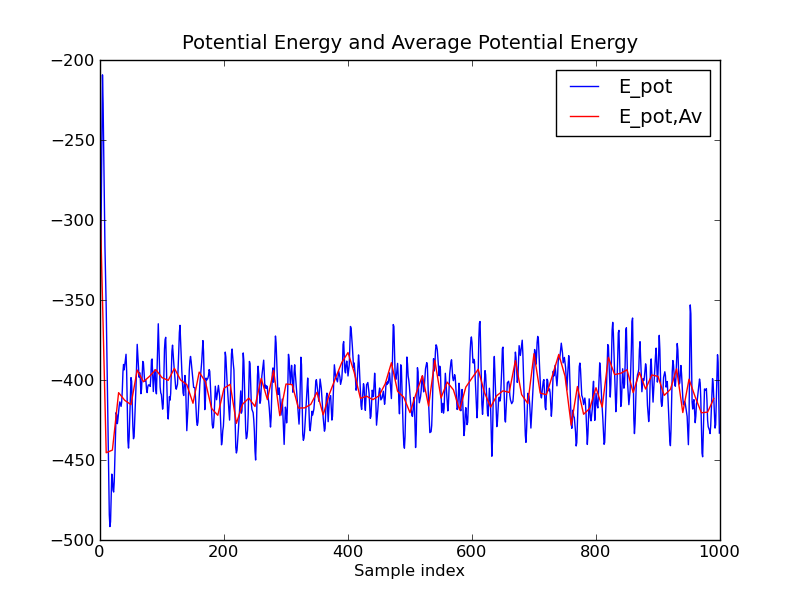
\includegraphics[width=0.75\textwidth]{potential_energy.png}
    \caption{Potential energy during a "healthy" MD simulation in a Lennard-Jones potential.}
    \label{fig:potential_energy}
\end{center}
\end{figure}


\newpage

If you finish early, do these exercises before you leave:\\

Multiply the random velocities in the initialize\_particles function by a small
scaling factor (i.e. a small number $< 1$).
This lowers the average velocities of the particles and corresponds to running
the simulation at a lower temperature.
Recall the Maxwell-Boltzmann distribution of the mean speed of
particles in a gas:

\begin{align}
    \langle v \rangle = \sqrt{ \frac{8\ R \ T}{\pi\ M}}
\end{align}

Here $R$ is the gas constant, $T$ the temperature and $M$ the molar mass of the
gas.\\

Answer the following two questions:

\begin{enumerate}
    \item Can you find a scaling factor so the particles behave more like a liquid rather than a gas? 
    \item What property of the Lennard-Jones is very important if you want to simulate aggregation of particles?
\end{enumerate}


% ***************************************************
% END DOCUMENT
% ***************************************************

\end{document}

